\documentclass[11pt,letterpaper]{article}
\usepackage{fullpage}
\usepackage[top=2cm, bottom=4.5cm, left=2.5cm, right=2.5cm]{geometry}
\usepackage{amsmath,amsthm,amsfonts,amssymb,amscd}
\usepackage{lastpage}
\usepackage{fancyhdr}
\usepackage{mathrsfs}
\usepackage{physics}
\usepackage{todonotes} 
\usepackage{siunitx}
\usepackage{subfiles}
\usepackage{float}
\usepackage{hyperref}
\usepackage{enumitem}
\usepackage{emoji}
\usepackage{url}
\hypersetup{colorlinks,breaklinks,
            urlcolor=[RGB]{0,0.5,0.5},
            linkcolor=[RGB]{0,0.5,0.5}}

\setlength{\parindent}{0.0in}
\setlength{\parskip}{0.05in}

\begin{document}

\thispagestyle{fancyplain}
\headheight 35pt
\author{}
\title{(Unofficial) UBC PHAS Comprehensive 2022 Solutions}
\date{\today}
\rfoot{\small\thepage}
\headsep 1.5em

\maketitle

\section*{S P H E R E}

\begin{center}
    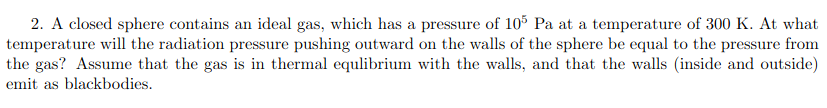
\includegraphics[width=\textwidth]{images/Q2.png}
\end{center}


Let's use little $p$ for pressure. $p = \SI{1e5}{Pa}$ at $T = \SI{300}{K}$.

Ideal gas, so initially:
\begin{align*}
    pV &= NkT \\
    \frac{p_0}{T_0} &= \frac{Nk}{V} \\
\end{align*}

And after changing temperature:
\begin{align*}
    p &= \frac{NkT}{V} \\
\end{align*}


Black-body power radiated: $P = A \sigma T^4$, where $\sigma = \SI{5.67e-8}{W m^{-2} K^{-4}}$ (on the formula sheet).

Here, $A = 4\pi R^2$ (surface area of sphere).

$P = 4\pi R^2 \sigma T^4$.

\newpage

Radiation pressure:
\todo[inline]{Honestly there might be an extra factor of two somewhere here, I forget?}
\begin{align*}
    p &= \frac{I}{c} \\
    &= \frac{\left(\frac{P}{A}\right)}{c} \\
    &= \frac{\left(\frac{P}{4\pi R^2}\right)}{c} \\
    &= \frac{\left(\frac{4\pi R^2 \sigma T^4}{4\pi R^2}\right)}{c} \\
    &= \frac{\sigma T^4}{c} \\
\end{align*}

When will this be equal to the pressure from the gas? Set our expressions equal:

\begin{align*}
    \frac{NkT}{V} &= \frac{\sigma T^4}{c} \\
    \frac{Nk}{V} \frac{c}{\sigma} &= T^3 \\
    \sqrt[3]{\frac{p_0}{T_0} \frac{c}{\sigma}} &= T = \SI{1.2e6}{K}\\
\end{align*}


\todo[inline]{Key take-aways:

    Note: had to look up the radiation pressure / blackbody stuff

    Ideal gas: $pV = NkT$

    Blackbody total power radiated: $P = A \sigma T^4$

    Radiation pressure: $p = \frac{I}{c}$}

\end{document}
